\documentclass[border=6pt]{standalone}
% Shared preamble of every figure (included by each fig*.tex)
\usepackage{fontspec}
\setmainfont{DejaVu Sans}
\setmonofont{DejaVu Sans Mono}
\usepackage{amsmath,amssymb}
\usepackage{tikz}
\usetikzlibrary{positioning,arrows.meta,fit,calc,decorations.pathreplacing,shapes.geometric,backgrounds}
\definecolor{cdata}{HTML}{4C78A8}
\definecolor{cmodel}{HTML}{F58518}
\definecolor{chead}{HTML}{54A24B}
\definecolor{cgold}{HTML}{E45756}
\definecolor{cgrey}{HTML}{9D9D9D}
\definecolor{cfull}{HTML}{B279A2}
\tikzset{
  box/.style={draw, rounded corners=2pt, align=center, inner sep=4pt, font=\small, minimum height=8mm},
  data/.style={box, fill=cdata!15, draw=cdata!80!black},
  model/.style={box, fill=cmodel!18, draw=cmodel!80!black},
  head/.style={box, fill=chead!18, draw=chead!70!black},
  note/.style={font=\footnotesize, align=center, text=black!70},
  arr/.style={-{Stealth[length=2.2mm]}, thick, black!70},
}

\begin{document}
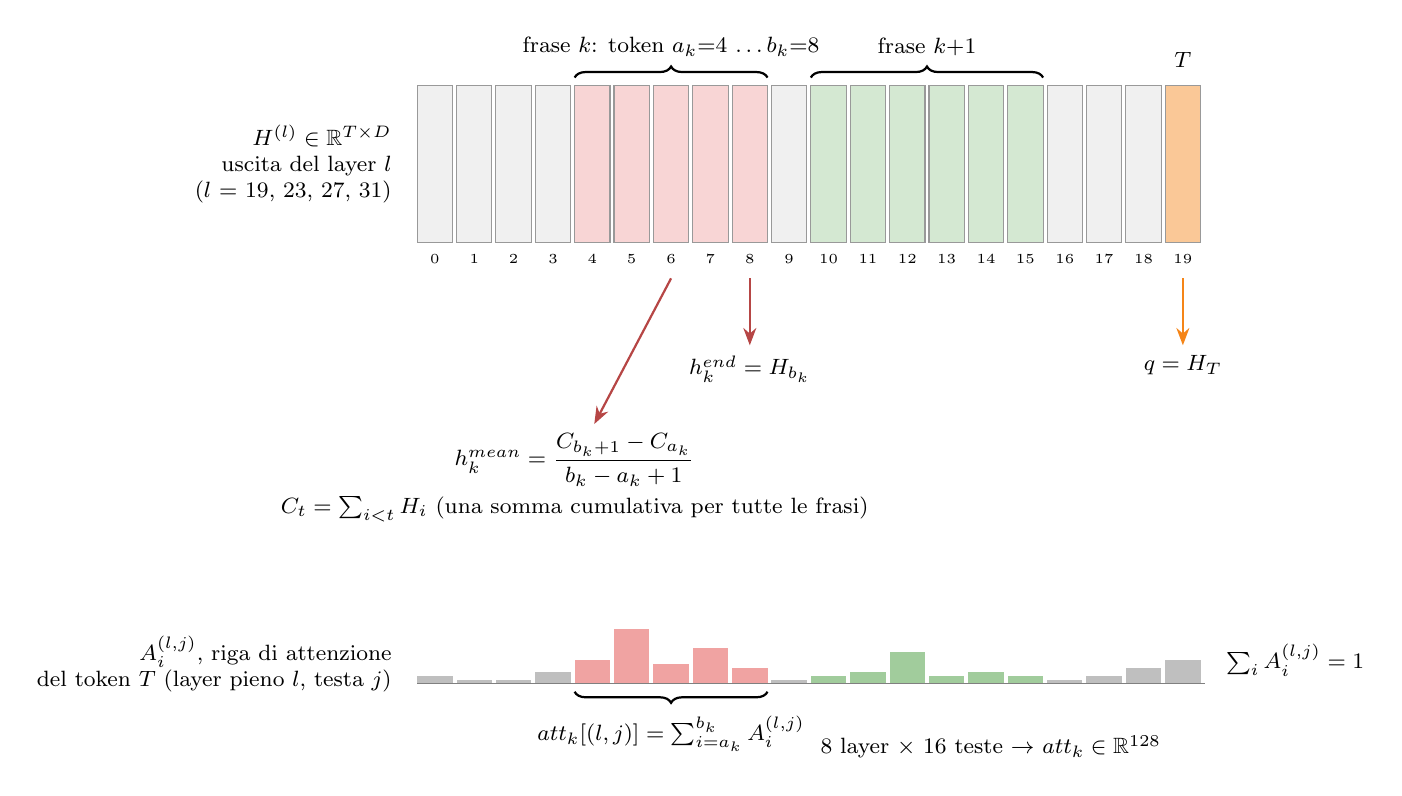
\begin{tikzpicture}[x=5mm,y=5mm]
% hidden states matrix: columns = tokens (0..19), rows = D
\node[anchor=east, font=\footnotesize, align=right] at (-0.4,2) {$H^{(l)} \in \mathbb{R}^{T \times D}$\\uscita del layer $l$\\($l$ = 19, 23, 27, 31)};
\foreach \t in {0,...,19}{
  \pgfmathsetmacro{\col}{ifthenelse(\t>=4 && \t<=8, 1, ifthenelse(\t>=10 && \t<=15, 2, 0))}
  \ifdim\col pt=1pt \def\fc{cgold!25}\else\ifdim\col pt=2pt \def\fc{chead!25}\else\def\fc{black!6}\fi\fi
  \fill[\fc, draw=black!40] (\t,0) rectangle ++(0.9,4);
  \node[font=\tiny] at (\t+0.45,-0.4) {\t};
}
\fill[cmodel!45, draw=black!40] (19,0) rectangle ++(0.9,4);
\draw[decorate, decoration={brace, amplitude=4pt}, thick] (4,4.2) -- node[above=4pt, font=\footnotesize] {frase $k$: token $a_k$=4 \dots $b_k$=8} (8.9,4.2);
\draw[decorate, decoration={brace, amplitude=4pt}, thick] (10,4.2) -- node[above=4pt, font=\footnotesize] {frase $k{+}1$} (15.9,4.2);
\node[font=\footnotesize, anchor=south] at (19.45,4.2) {$T$};
% h_end
\draw[arr, cgold!80!black] (8.45,-0.9) -- (8.45,-2.6) node[below, font=\footnotesize, text=black] {$h^{end}_k = H_{b_k}$};
% h_mean via cumsum
\draw[arr, cgold!80!black] (6.45,-0.9) -- (4.5,-4.6);
\node[font=\footnotesize, anchor=north, align=center] at (4,-4.6) {$h^{mean}_k = \dfrac{C_{b_k+1}-C_{a_k}}{b_k-a_k+1}$\\[1mm]$C_t=\sum_{i<t} H_i$ (una somma cumulativa per tutte le frasi)};
\draw[arr, cmodel] (19.45,-0.9) -- (19.45,-2.6) node[below, font=\footnotesize, text=black] {$q = H_T$};
% attention row
\begin{scope}[yshift=-5.6cm]
\node[anchor=east, font=\footnotesize, align=right] at (-0.4,0.5) {$A^{(l,j)}_{i}$, riga di attenzione\\del token $T$ (layer pieno $l$, testa $j$)};
\foreach \t/\h in {0/0.2,1/0.1,2/0.1,3/0.3,4/0.6,5/1.4,6/0.5,7/0.9,8/0.4,9/0.1,10/0.2,11/0.3,12/0.8,13/0.2,14/0.3,15/0.2,16/0.1,17/0.2,18/0.4,19/0.6}{
  \pgfmathsetmacro{\col}{ifthenelse(\t>=4 && \t<=8, 1, ifthenelse(\t>=10 && \t<=15, 2, 0))}
  \ifdim\col pt=1pt \def\fc{cgold!55}\else\ifdim\col pt=2pt \def\fc{chead!55}\else\def\fc{black!25}\fi\fi
  \fill[\fc] (\t,0) rectangle ++(0.9,\h);
}
\draw[black!50] (0,0) -- (20,0);
\node[font=\footnotesize, anchor=west] at (20.3,0.6) {$\sum_i A^{(l,j)}_i = 1$};
\draw[decorate, decoration={brace, amplitude=4pt, mirror}, thick] (4,-0.2) -- node[below=5pt, font=\footnotesize] {$att_k[(l,j)] = \sum_{i=a_k}^{b_k} A^{(l,j)}_i$} (8.9,-0.2);
\node[font=\footnotesize, anchor=west, align=left] at (10,-1.6) {8 layer $\times$ 16 teste $\to$ $att_k\in\mathbb{R}^{128}$};
\end{scope}
\end{tikzpicture}
\end{document}
